\documentclass{beamer}


\usepackage[spanish]{babel}
\usepackage[T1]{fontenc}
\usepackage[utf8]{inputenc}

\usepackage{graphics}
\graphicspath{{img/}}

\usetheme{Madrid}
\usecolortheme{beaver}
\setbeamercovered{transparent}

% \usepackage{beamerthemesplit} // Activate for custom appearance

\title{Modelación Basada en Agentes}
\author{Dr. Felipe Contreras}
\date{\today}

\begin{document}

\frame{\titlepage}

\section[Outline]{}
\frame{\tableofcontents}

\section{Antecedentes}

\subsection{Sistemas Complejos}
\frame{\alert{Sistemas Complejos}}
  \setbeamercovered{transparent}
\begin{frame}[t]
  \frametitle{Características}
  \begin{itemize}[<+-| alert@+>]
  \item Sistema: Conjunto de elementos o partes conectadas entre sí, que llevan acabo cierta función
  \item Complejo $\neq$ Complicado
  \item Presentan auto-organización
  \item Exhiben propiedades emergentes (``el todo es más que la suma de sus partes'')
  \begin{enumerate}[<+-| alert@+>]
  \item Muchos elementos
  \item Las interacciones son dinámicas
  \item Elementos influyen y son influidos por los demás
  \item Las interacciones son no lineales (pequeñas ``causas'', pueden tener ``efectos'' grandes)
  \item Las interacciones son recursivas
  \item Son abiertos % interacturan con otros sistemas
  \item Operan lejos del equilibrio
  \item Tienen una historia
  \item Los elementos actúan con información local
  \end{enumerate}
  \end{itemize}
  \end{frame}

\subsection{Mapeos Discretos}
\frame{\alert{Mapeos Discretos}}
\frame{
  \frametitle{Mapeos discretos}
  \begin{itemize}[<+->]
  \item $y = f(x)$
  \item $x_{1} = f(x_{0})$
  \item $x_{2} = f(x_{1}), x_{3}=f(x_{2}), x_{4} = f(x_{3}), ...$
  \end{itemize}
}
\frame{\frametitle{Representación gráfica}
\begin{block}{}
\begin{center}
\includegraphics<+>[height=.5\textheight]{mapeo1}
\includegraphics<+>[height=.5\textheight]{mapeo2}
\includegraphics<+>[width=.8\textwidth]{mapeo3}
\end{center}
\end{block}
}
\frame
{
  \frametitle{Características}

  \begin{itemize}[<+->]
  \item Converge (a un punto)
  \item No converge: tiene ciclo límite
  \item No converge: órbita densa
  \end{itemize}
}

\subsection{Autómatas Celulares}
\frame{\alert{Autómatas Celulares}}
\begin{frame}[t]
  \frametitle{Definición}
  \begin{columns}[t]
  \column{.5\textwidth}
  \begin{block}{}
	\begin{itemize}[<+->]
		\item Vocabulario $\sigma$ de $n$ símbolos
		\item Organización de $m$ de estos símbolos en un estado inicial $E_{0}$
		\item Tamaño de vecindad o radio $\rho$
		\item Condiciones en la frontera (cíclica, terminación, valor único)
		\item Regla de evolución (función de mapeo)
	\end{itemize}
  \end{block}
   \column{.5\textwidth}
  \begin{center}
	\only<1> {$\sigma = \{0, 1\}$, $n=2$}
	\includegraphics<2>[width=.9\textwidth]{automata1}
	\only<3> {$\rho=3$}
	\includegraphics<4>[width=.9\textwidth]{automata2}
	\includegraphics<5>[height=.4\textheight]{automata3}
  \end{center}
  \end{columns}
\end{frame}

\begin{frame}[t]
  \frametitle{Regla de evolución}
  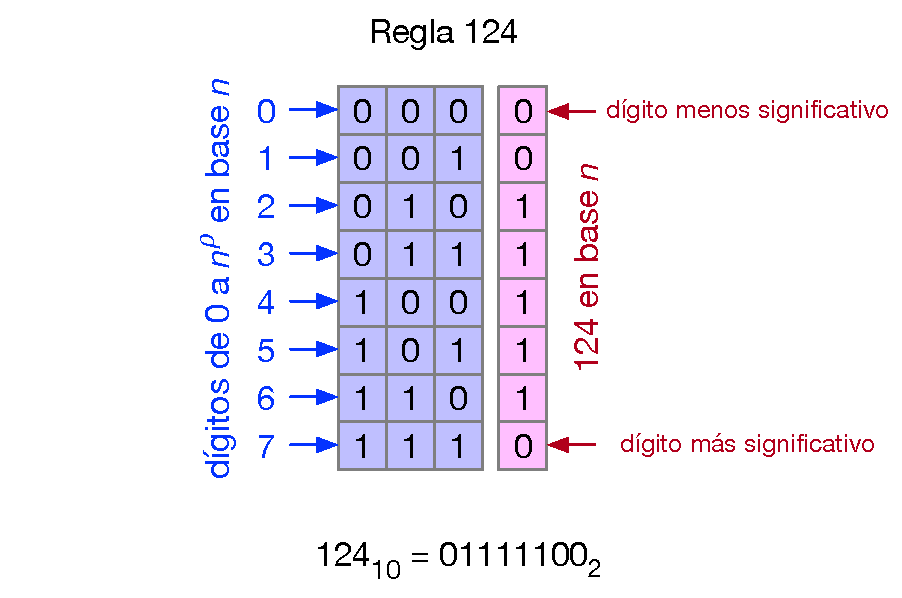
\includegraphics[width=.9\textwidth]{automata4}
\end{frame}

\begin{frame}[t]
  \frametitle{Aplicación de la regla}
  \includegraphics<+>[width=.9\textwidth]{automata51}
  \includegraphics<+>[width=.9\textwidth]{automata52}
  \includegraphics<+>[width=.9\textwidth]{automata53}
  \includegraphics<+>[width=.9\textwidth]{automata54}
  \includegraphics<+>[width=.9\textwidth]{automata55}
  \includegraphics<+>[width=.9\textwidth]{automata56}
  \includegraphics<+>[width=.9\textwidth]{automata57}
  \includegraphics<+>[width=.9\textwidth]{automata58}
  \includegraphics<+>[width=.9\textwidth]{automata59}
  \only<+>{?`cómo quedan las demás?, ?`cómo funciona la condición de frontera cíclica?}
\end{frame}

\begin{frame}[t]
  \frametitle{Ejemplos}
  \begin{center}
  \only<+> {Regla 90, $E_{0}$=``central'' }
  \only<+> {Regla 94, $E_{0}$=``01110000000000001111100001111'' }
  \only<+> {Regla 135, $E_{0}$=``azar'' }
  \end{center}
  \begin{center}
  \includegraphics<1>[height=.6\textheight]{ac11}
  \includegraphics<2>[height=.6\textheight]{ac12}
  \includegraphics<3>[height=.6\textheight]{ac13}
  \end{center}
\end{frame}

\begin{frame}[t]
\frametitle{Categorías}
\begin{itemize}[<+->]
	\item 
\end{itemize}
\end{frame}

\begin{frame}[t]
  \frametitle{Autómatas en 2D: El juego de la vida}
  \begin{itemize}[<+->]
  \item {El conjunto de símbolos es $\sigma=\{0,1\}$, significando 0=``muerta'', 1=``viva''}
  \item {$E_{0}$, y todos los demás estados, están dispuestos en una parrilla 2D de celdas}
  \item {La vecindad mide $\rho=(3,3)$, es un cuadro de $3\times 3$ símbolos}
  \item {La regla de evolución para el siguiente estado, asigna a la celda central el valor:}
  \begin{itemize}[<+->]
  \item ``viva'', si la celda central esta ``muerta'' y hay exactamente 3 vecinos vivos
  \item ``muerta'', si la celda central está ``viva'' y más de 3 (sobrepoblación) o menos de 2 (soledad) vecinos están vivos
  \item En cualquier otro caso, la celda mantiene su símbolo
  \end{itemize}
  \end{itemize}
  \begin{center}\includegraphics<+>[width=.6\textwidth]{vida1}\end{center}
\end{frame}

\end{document}